Zu Beginn wird eine Gegenspannung $U_\su{G}$ bei maximalem Heizstrom $I_\su{f} = \SI{2,5}{\ampere}$
angelegt. Die Spannung wird dabei von $U_\su{G} = (0-1)\,\si{\volt}$ hochgeregelt. Die entsprechenden
Werte bedfinden sich in Tabelle \ref{tab:gegen}.
\begin{table}[H]
  \centering
  \caption{Gemessener Strom $I_\su{G}$ in Abhängigkeit der Gegenspannung $U_\su{G}$.}
  \begin{tabular}{cc}
    \toprule
    \mc{1}{c}{Gegenspannung} & \mc{1}{c}{Strom} \\
    $U_\su{G}\,/\,\si{\volt}$ & $I_\su{G}\,/\,\si{\nano\ampere}$ \\
    \midrule
    0.00  & 69.0  \\
    0.04  & 59.0  \\
    0.08  & 53.0  \\
    0.12  & 46.0  \\
    0.16  & 38.0  \\
    0.20  & 33.0  \\
    0.24  & 28.0  \\
    0.28  & 25.0  \\
    0.32  & 22.0  \\
    0.36  & 19.0  \\
    0.40  & 16.0  \\
    0.44  & 14.0  \\
    0.48  & 12.0  \\
    0.52  & 10.0  \\
    0.56  &  9.0  \\
    0.60  &  7.0  \\
    0.64  &  6.5  \\
    0.68  &  5.5  \\
    0.72  &  4.5  \\
    0.76  &  3.5  \\
    0.80  &  3.0  \\
    0.84  &  2.5  \\
    0.88  &  2.0  \\
    0.92  &  1.5  \\
    0.96  &  1.0  \\
    1.00  &  0.5  \\
    \bottomrule
  \end{tabular}
  \label{tab:gegen}
\end{table}
Aus diesen Werten wird die Temperatur $T$ mittels
\begin{equation}
  T = -\frac{e_0}{ka}
\end{equation}
aus Gleichung \eqref{eqn:T} berechnet.
Dazu wird $\log{\left(\frac{I_\su{G}}{I_\su{max}}\right)}$ gegen $U_\su{G}$ in Abbildung \ref{fig:g} aufgetragen.
Hierbei gilt $I_\su{max} = \SI{69}{\nano\ampere}$ - der maximale Strom, ohne Gegenspannung.
\begin{figure}[H]
  \centering
  \includegraphics[width=0.8\textwidth]{bilder/Kathodentemperatur.pdf}
  \caption{Strom in Abhängigkeit der Gegenspannung zur Bestimmung der Temperatur.}
  \label{fig:g}
\end{figure}
Daraus ergeben sich die Parameter
\begin{align}
  a &= \SI[per-mode=fraction]{-4,1\pm0,2}{\per\volt}\\ \notag
  b &= 0,03\pm0,09.\\ \notag
\end{align}
Somit folgt für die Temperatur
\begin{equation}
  T = \SI{2810\pm140}{\kelvin}. \notag
\end{equation}
Anschließend wird die Spannung am Kondensator umgepolt. Es werden zu fünf verschiedenen
Heizströmen $I_\su{f}$ mit der jeweiligen Heizspannung $U_\su{f}$ die Ströme $I$
in Abhängigkeit der angelegten Anodenspannung $U_\su{A}$ aufgenommen.
Die Werte zu dieser Messung befinden sich in Tabelle \ref{tab:anode}.
\begin{table}[H]
  \centering
  \caption{Gemessener Strom $I$ in Abhängigkeit der Anodenspannung $U_\su{A}$.}
  \begin{tabular}{c|ccccc}
    \toprule
    \mc{1}{c|}{Anodenspannung} & \mc{5}{c}{Strom} \\
    $U_\su{A}\,/\,\si{\volt}$ & $I_1\,/\,\si{\nano\ampere}$ & $I_2\,/\,\si{\nano\ampere}$ & $I_3\,/\,\si{\nano\ampere}$ & $I_4\,/\,\si{\nano\ampere}$ & $I_5\,/\,\si{\nano\ampere}$ \\
    \midrule
     0 & 0 &  0 &  0 &   0 &    0 \\
     5 & 0 &  0 &  0 &   0 &    8 \\
    10 & 2 &  0 & 11 &   7 &   50 \\
    15 & 5 &  6 & 28 &  34 &  112 \\
    20 & 6 & 14 & 46 &  75 &  192 \\
    25 & 7 & 19 & 54 & 124 &  287 \\
    30 & 7 & 22 & 58 & 202 &  396 \\
    35 & 7 & 23 & 60 & 227 &  503 \\
    40 & 8 & 24 & 61 & 243 &  603 \\
    45 & 8 & 24 & 62 & 250 &  692 \\
    50 & 8 & 25 & 63 & 254 &  782 \\
    60 & 8 & 25 & 64 & 259 &  942 \\
    70 & 8 & 25 & 64 & 263 & 1073 \\
    80 & 8 & 25 & 65 & 266 & 1165 \\
    90 & 8 & 26 & 65 & 268 & 1220 \\
   100 & 9 & 26 & 66 & 269 & 1257 \\
   110 & 9 & 26 & 66 & 271 & 1285 \\
   120 & 9 & 26 & 66 & 272 & 1301 \\
   130 & 9 & 26 & 67 & 273 & 1313 \\
   140 & 9 & 26 & 67 & 274 & 1321 \\
   150 & 9 & 27 & 67 & 275 & 1329 \\
   160 & 9 & 27 & 67 & 276 & 1335 \\
   170 & 9 & 27 & 68 & 277 & 1340 \\
   180 & 9 & 27 & 68 & 278 & 1345 \\
   190 & 9 & 27 & 68 & 279 & 1350 \\
   200 & 9 & 27 & 68 & 280 & 1354 \\
   210 & 9 & 27 & 69 & 280 & 1358 \\
   220 & 9 & 27 & 69 & 281 & 1361 \\
   230 & 9 & 27 & 69 & 282 & 1364 \\
   240 & 9 & 27 & 69 & 282 & 1368 \\
   250 & 9 & 27 & 69 & 283 & 1372 \\
   \midrule
   $I_\su{f}$ & 1,8 & 1,9 & 2,0 & 2,2 & 2,4 \\
   $U_\su{f}$ & 3,9 & 4,0 & 4,2 & 5,0 & 6,0 \\
   \bottomrule
  \end{tabular}
  \label{tab:anode}
\end{table}
In Abbildung \ref{fig:kenn} wird dann der Strom $I$ gegen die korrigierte Spannung $U_\su{korr}$
dargestellt. Die Spannung $U_\su{A}$ wird korrigiert, da der Innenwiederstand
$R_\su{i} = \SI{1}{\mega\ohm}$ des Nanoamperemeters die Spannung zwischen
Anode und Kathode verändert. Die Korrektur erfolgt über
\begin{equation}
  U_\su{korr} = U_\su{A}-R_\su{i}\,\cdot\, I. \\
\end{equation}
\begin{figure}[H]
  \centering
  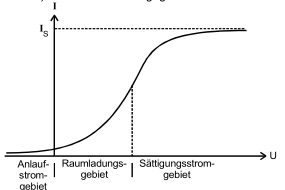
\includegraphics[width=0.8\textwidth]{bilder/kennlinie.pdf}
  \caption{Die Kennlinien des Wolframdrahtes zu fünf verschiedenen Heizleistungen.}
  \label{fig:kenn}
\end{figure}
Aus Abbildung \ref{fig:kenn} lassen sich die Sättigungsströme
\begin{align*}
  I_\su{s,1} &= \SI{10}{\nano\ampere}  \\
  I_\su{s,2} &= \SI{30}{\nano\ampere} \\
  I_\su{s,3} &= \SI{70}{\nano\ampere}  \\
  I_\su{s,4} &= \SI{280}{\nano\ampere}  \\
  I_\su{s,5} &= \SI{1370}{\nano\ampere}  \\
\end{align*}
mithilfe der Werte aus Tabelle \ref{tab:anode} ablesen.

Nun wird $\log{\left(\frac{I}{I_\su{s}}\right)}$ gegen $U_\su{A}$ in Grafik \ref{fig:langmuir}
aufgetragen.
\begin{figure}
  \centering
  \includegraphics[width=0.8\textwidth]{bilder/langmuir.pdf}
  \caption{Bestimmung des Exponenten der Strom-Spannungs-Beziehung.}
  \label{fig:langmuir}
\end{figure}
Hieraus ergeben sich die Parameter
\begin{align*}
  m &= \SI[per-mode=fraction]{0,07\pm0,01}{\per\volt} \\
  n &= -3,6\pm0,4. \\
\end{align*}
